\documentclass[10pt]{report}
\usepackage{float}
\usepackage{amsfonts}
\usepackage{amssymb}
\usepackage{amsmath}
\usepackage{makeidx}
\usepackage{amsgen}
\usepackage{epsf}
\usepackage{fancyhdr}
\usepackage{acro}
\usepackage{etoolbox}
\usepackage[hidelinks]{hyperref}
\usepackage{subfigure}
\usepackage{lastpage}
\usepackage{ltablex}
\usepackage{graphicx}
\usepackage{color}
\usepackage{url}
\usepackage[table]{xcolor}
\usepackage{multirow}
\usepackage{enumitem}
\usepackage{cite}
\usepackage{tikz}
\usepackage[latin1]{inputenc}
\usepackage[official]{eurosym}
\setlength{\hoffset}{0pt}
\setlength{\oddsidemargin}{0pt}
\setlength{\evensidemargin}{9pt}
\setlength{\marginparwidth}{54pt}
\setlength{\textwidth}{481pt}
\setlength{\voffset}{-18pt}
\setlength{\marginparsep}{7pt}
\setlength{\topmargin}{0pt}
\setlength{\headheight}{13pt}
\setlength{\headsep}{10pt}
\setlength{\footskip}{27pt}
\setlength{\textheight}{708pt}
\begin{document}
\title{The Middle Region in the OpenMod4Africa Madrid Workshop}
\maketitle
\newpage
\listoffigures
\newpage
\listoftables
\newpage
\tableofcontents
\newpage
\chapter{Installed Capacity}
\begin{figure}[H]
\centering
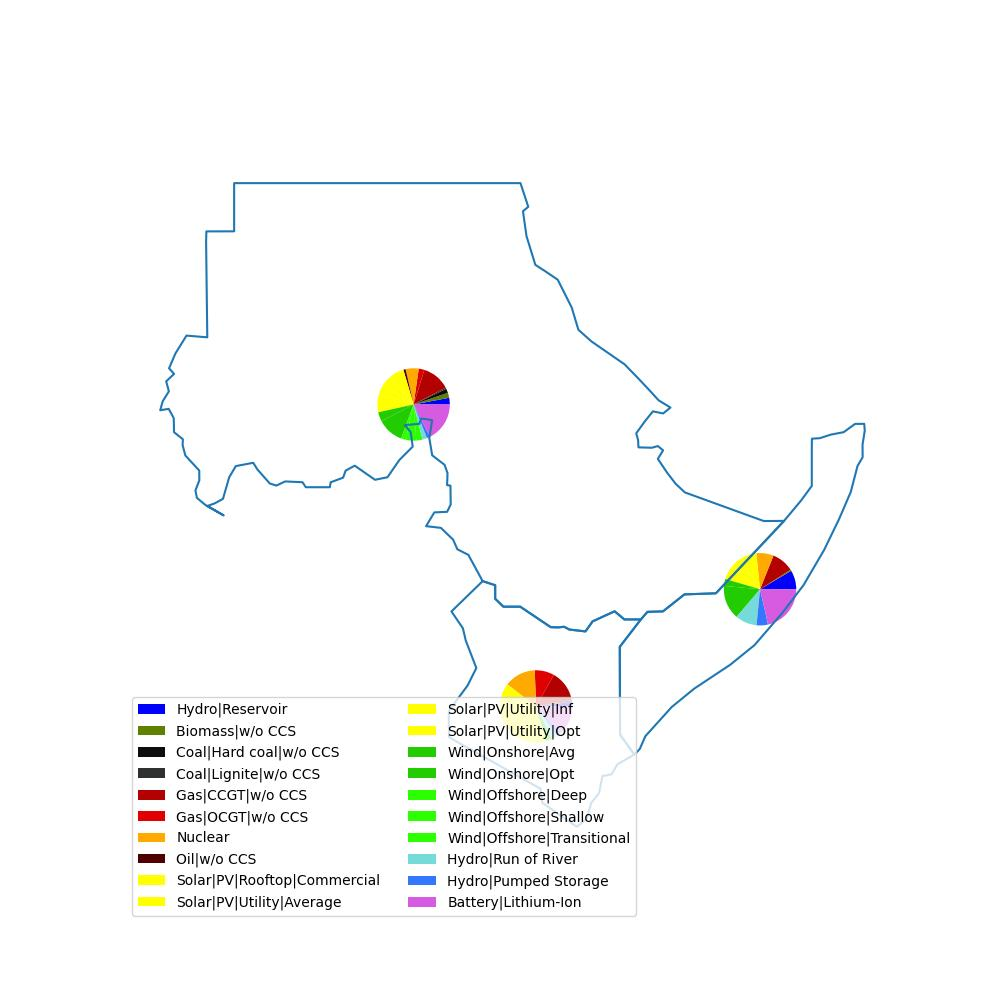
\includegraphics[width=\textwidth,keepaspectratio]{\home\Plan4Res\P4R3\p4r-env\bin\..\data\local\LoR_Madrid\results_simul\IMG\InstalledCapacityMapPieEurope.jpeg}
\caption{Map of Installed Capacity (Pies)}
\label{fig:InstalledCapacityMapPieEurope.jpeg}
\end{figure}
\begin{figure}[H]
\centering
\includegraphics[width=\textwidth,keepaspectratio]{\home\Plan4Res\P4R3\p4r-env\bin\..\data\local\LoR_Madrid\results_simul\IMG\InstalledCapacityMapBarEurope.jpeg}
\caption{Map of Installed Capacity (MW)}
\label{fig:InstalledCapacityMapBarEurope.jpeg}
\end{figure}
\begin{figure}[H]
\centering
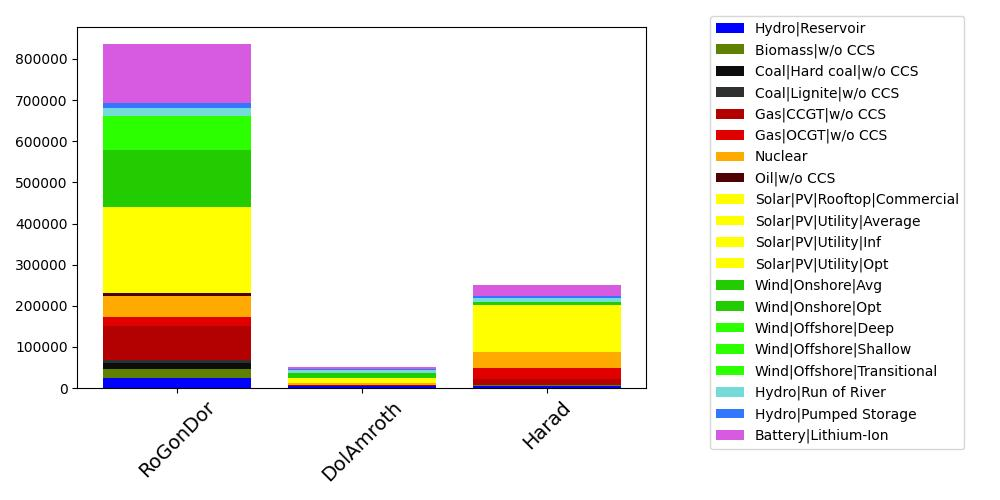
\includegraphics[width=\textwidth,keepaspectratio]{\home\Plan4Res\P4R3\p4r-env\bin\..\data\local\LoR_Madrid\results_simul\IMG\InstalledCapacityBar.jpeg}
\caption{Installed Capacity (MW)}
\label{fig:InstalledCapacityBar.jpeg}
\end{figure}
\begin{figure}[H]
\centering
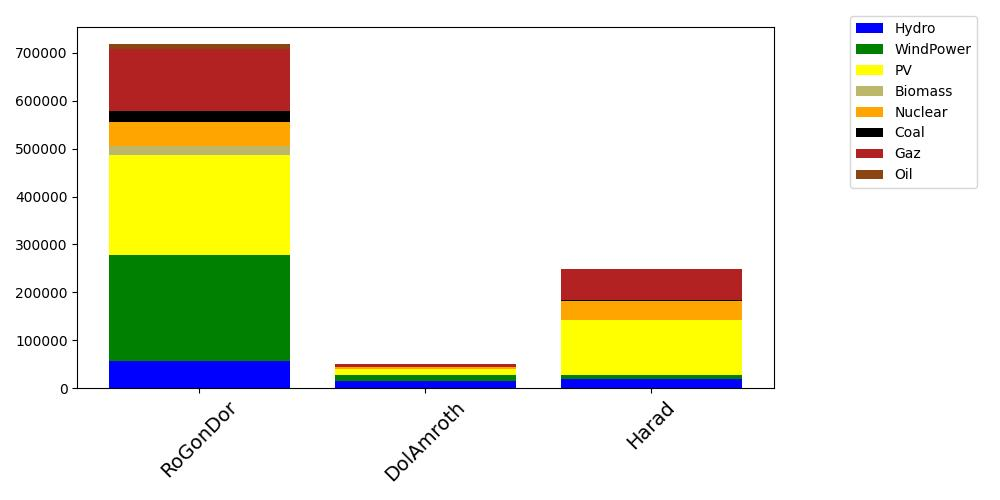
\includegraphics[width=\textwidth,keepaspectratio]{\home\Plan4Res\P4R3\p4r-env\bin\..\data\local\LoR_Madrid\results_simul\IMG\AggrInstalledCapacityBar.jpeg}
\caption{Installed Aggregated Capacity (MW)}
\label{fig:AggrInstalledCapacityBar.jpeg}
\end{figure}
\chapter{Stochastic Results}
\section{Demand}
\begin{figure}[H]
\centering
\includegraphics[width=\textwidth,keepaspectratio]{\home\Plan4Res\P4R3\p4r-env\bin\..\data\local\LoR_Madrid\results_simul\IMG\Demand.jpeg}
\caption{Demands for all scenarios (MWh)}
\label{fig:Demand.jpeg}
\end{figure}
\section{Marginal Costs}
\begin{figure}[H]
\centering
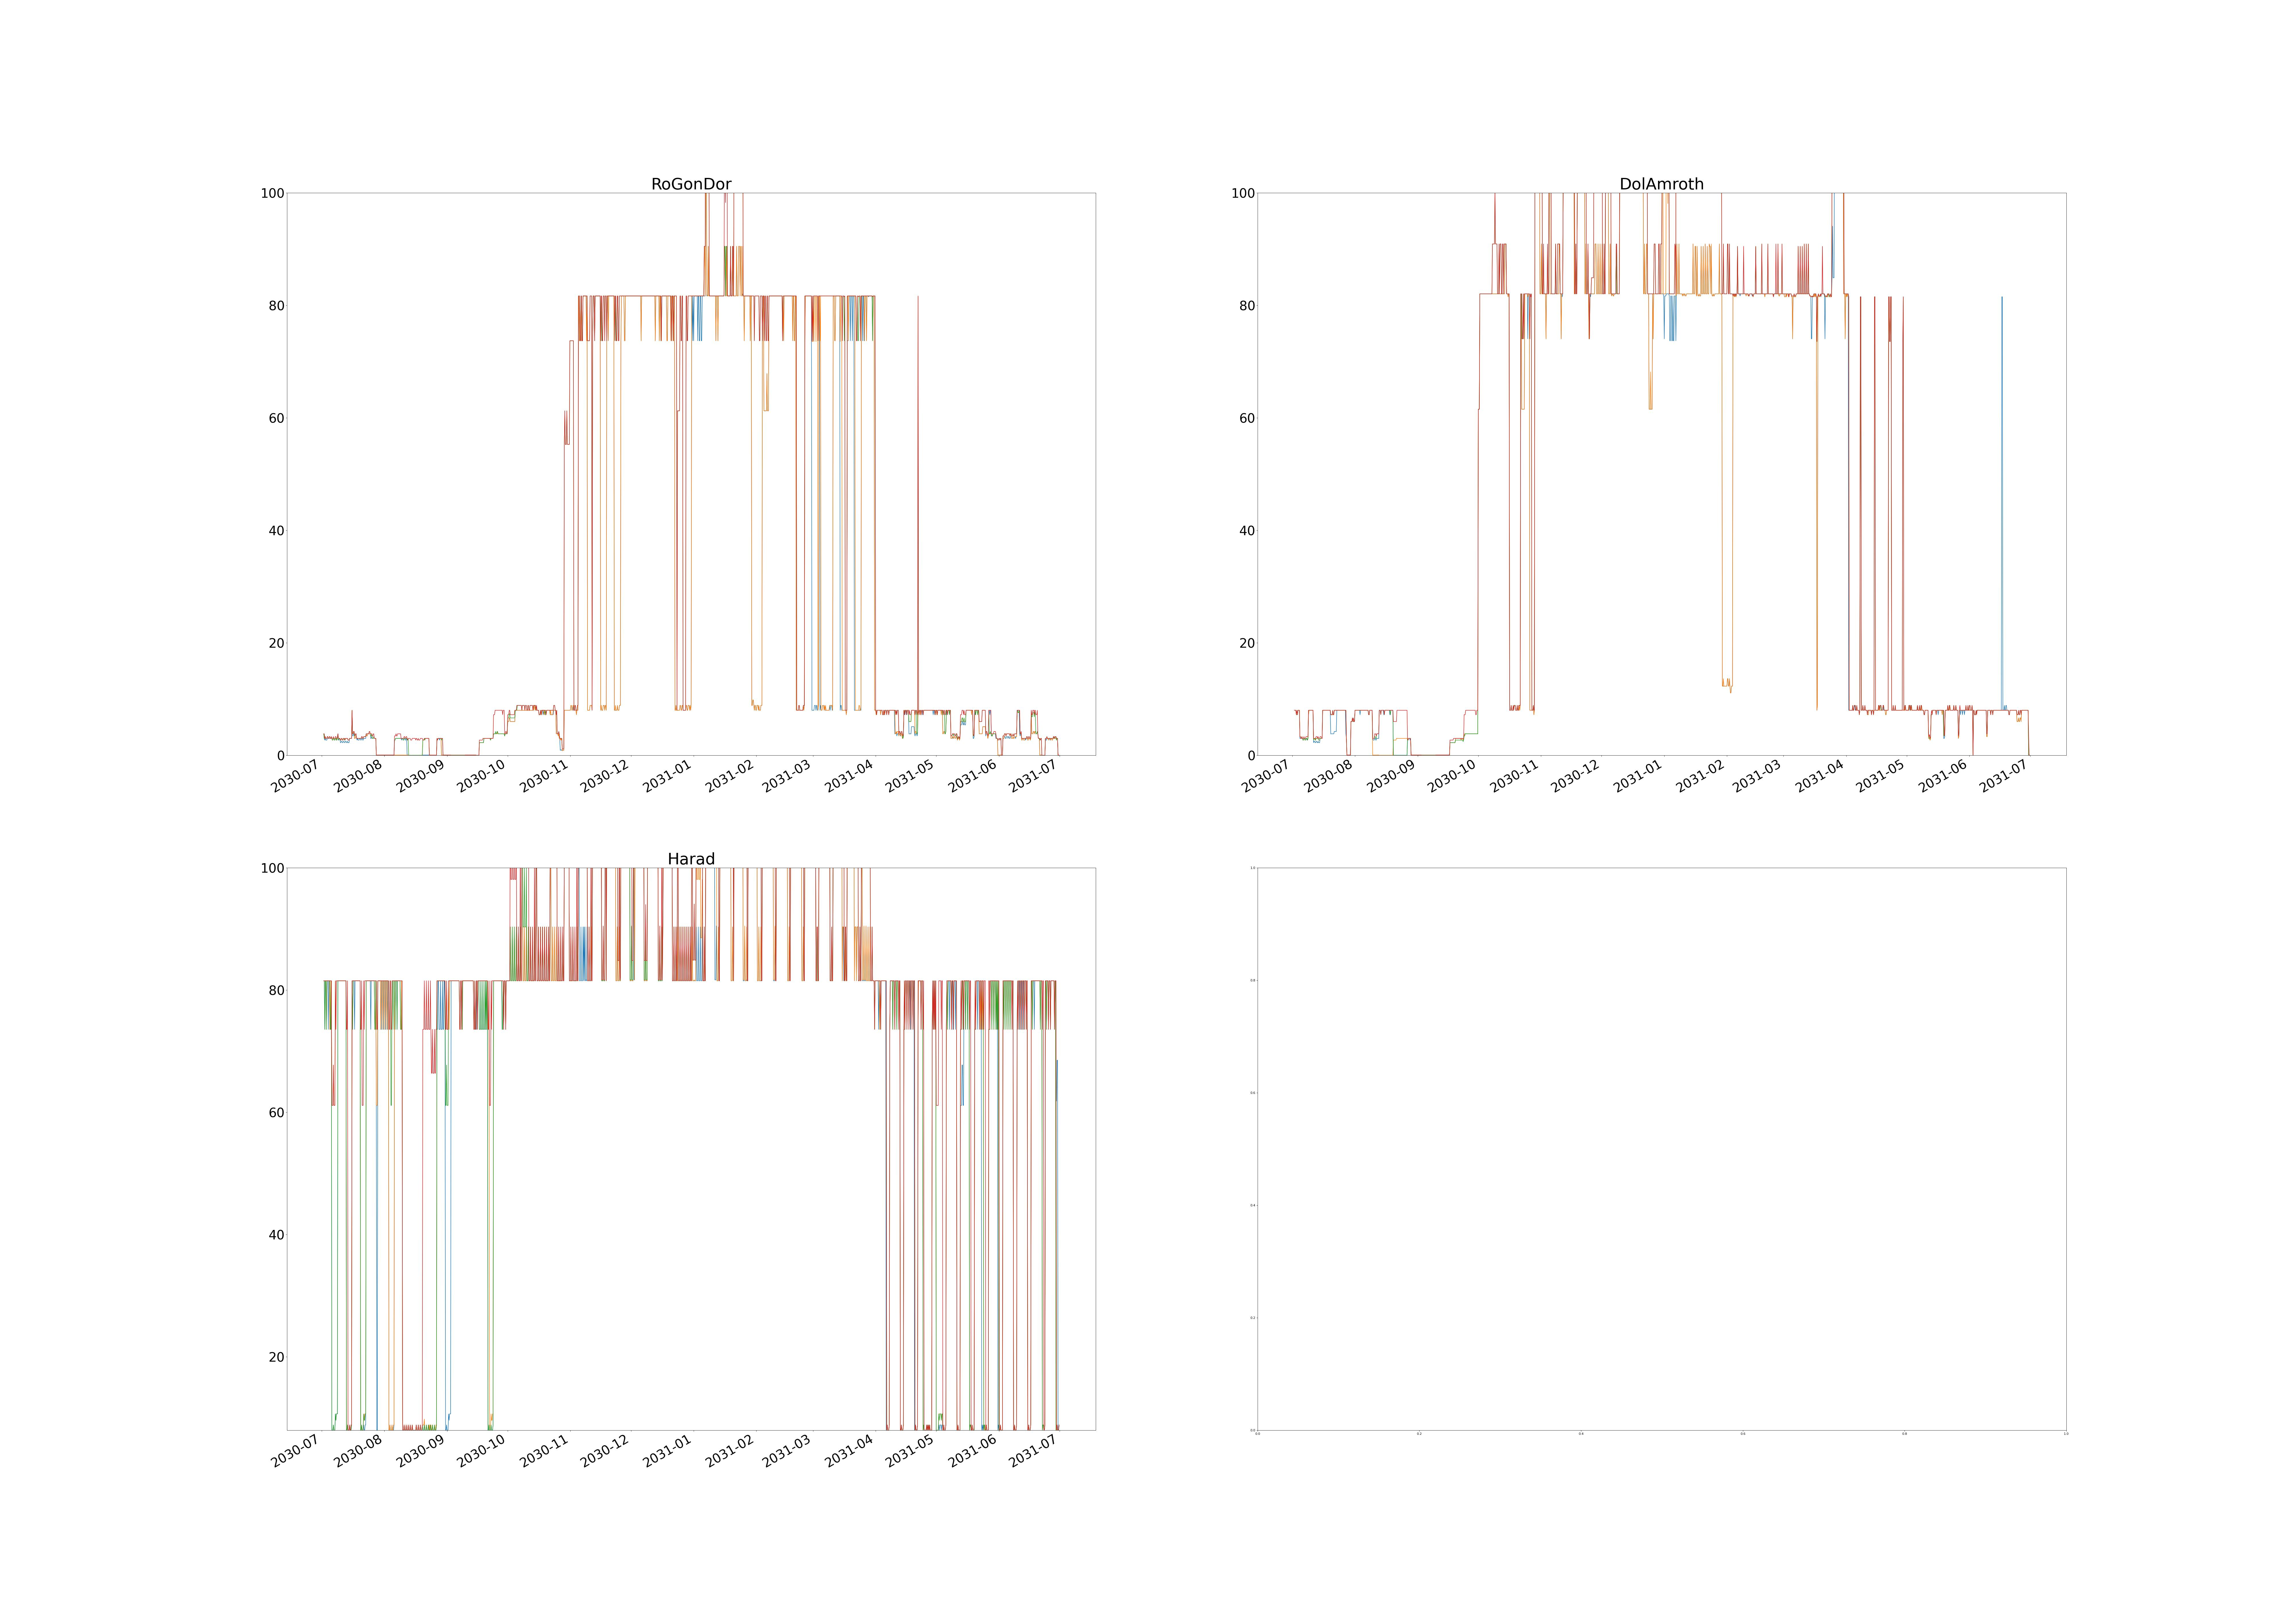
\includegraphics[width=\textwidth,keepaspectratio]{\home\Plan4Res\P4R3\p4r-env\bin\..\data\local\LoR_Madrid\results_simul\IMG\MarginalCostActivePowerDemand.jpeg}
\caption{Marginal Costs for all scenarios (Euro/MWh)}
\label{fig:MarginalCostActivePowerDemand.jpeg}
\end{figure}
\begin{figure}[H]
\centering
\includegraphics[width=\textwidth,keepaspectratio]{\home\Plan4Res\P4R3\p4r-env\bin\..\data\local\LoR_Madrid\results_simul\IMG\HistCmar.jpeg}
\caption{Histograms of Marginal Costs for all scenarios (Euro/MWh)}
\label{fig:HistCmar.jpeg}
\end{figure}
\begin{figure}[H]
\centering
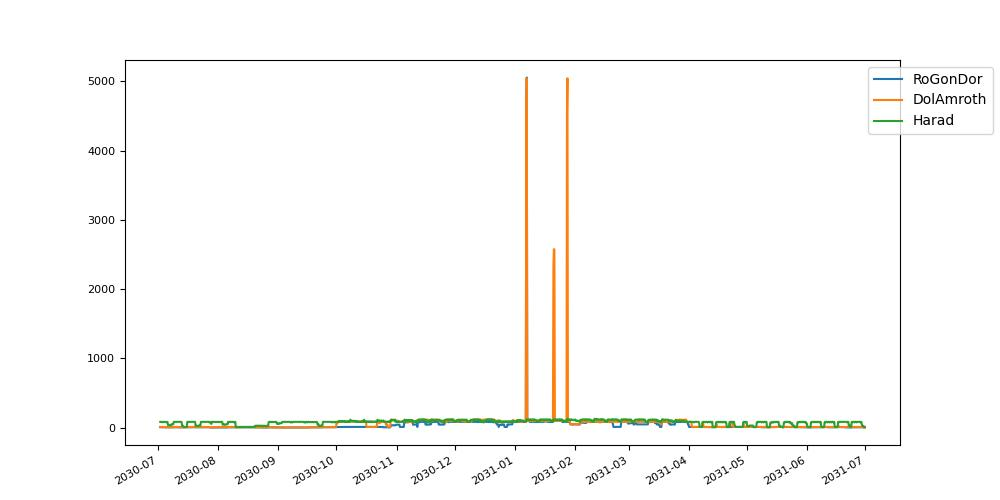
\includegraphics[width=\textwidth,keepaspectratio]{\home\Plan4Res\P4R3\p4r-env\bin\..\data\local\LoR_Madrid\results_simul\IMG\meanScenCmar.jpeg}
\caption{Mean Marginal Costs (Euro/MWh)}
\label{fig:meanScenCmar.jpeg}
\end{figure}
\begin{figure}[H]
\centering
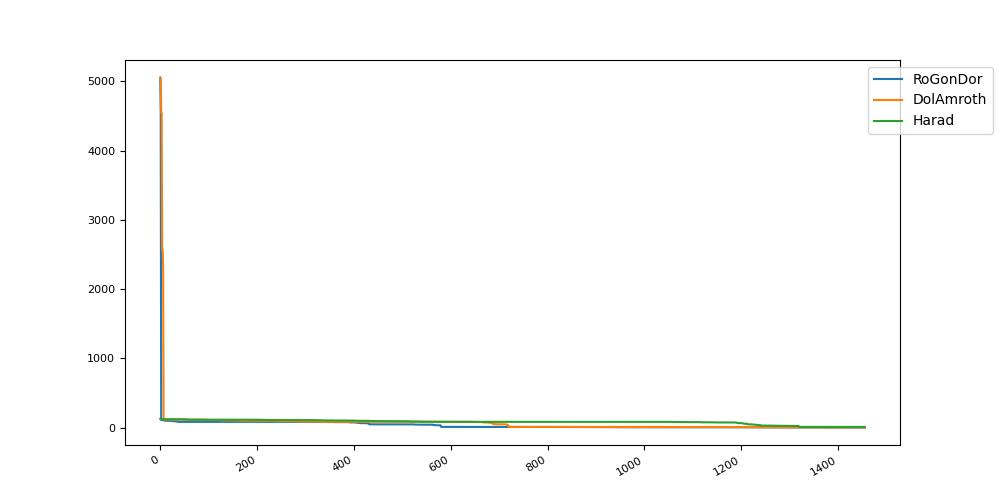
\includegraphics[width=\textwidth,keepaspectratio]{\home\Plan4Res\P4R3\p4r-env\bin\..\data\local\LoR_Madrid\results_simul\IMG\MonotoneCmar.jpeg}
\caption{Histogram of Mean Marginal Costs (Euro/MWh)}
\label{fig:MonotoneCmar.jpeg}
\end{figure}
\begin{figure}[H]
\centering
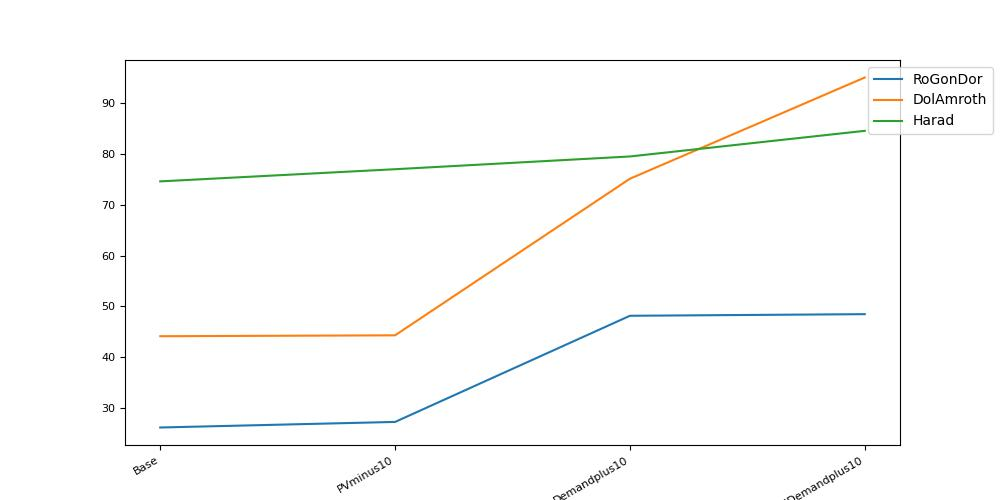
\includegraphics[width=\textwidth,keepaspectratio]{\home\Plan4Res\P4R3\p4r-env\bin\..\data\local\LoR_Madrid\results_simul\IMG\meanTimeCmar.jpeg}
\caption{Mean on all Timesteps of Marginal Costs per Scenario (Euro/MWh)}
\label{fig:meanTimeCmar.jpeg}
\end{figure}
\section{Volumes in seasonal storages}
\begin{figure}[H]
\centering
\includegraphics[width=\textwidth,keepaspectratio]{\home\Plan4Res\P4R3\p4r-env\bin\..\data\local\LoR_Madrid\results_simul\IMG\Volume-Reservoir.jpeg}
\caption{Volumes of seasonal storages (Resservoirs) (MWh)}
\label{fig:Volume-Reservoir.jpeg}
\end{figure}
\section{Mean Energy Generated}
\begin{figure}[H]
\centering
\includegraphics[width=\textwidth,keepaspectratio]{\home\Plan4Res\P4R3\p4r-env\bin\..\data\local\LoR_Madrid\results_simul\IMG\MeanEnergyMapPieEurope.jpeg}
\caption{Map of Mean Power Generation (MWh)}
\label{fig:MeanEnergyMapPieEurope.jpeg}
\end{figure}
\begin{figure}[H]
\centering
\includegraphics[width=\textwidth,keepaspectratio]{\home\Plan4Res\P4R3\p4r-env\bin\..\data\local\LoR_Madrid\results_simul\IMG\MeanEnergyBar.jpeg}
\caption{Mean Power Generation (MWh)}
\label{fig:MeanEnergyBar.jpeg}
\end{figure}
\begin{figure}[H]
\centering
\includegraphics[width=\textwidth,keepaspectratio]{\home\Plan4Res\P4R3\p4r-env\bin\..\data\local\LoR_Madrid\results_simul\IMG\ChloroMap-MeanEnergyAggr.jpeg}
\caption{Maps of Mean Generation per technology (MWh)}
\label{fig:ChloroMap-MeanEnergyAggr.jpeg}
\end{figure}
\section{Non Served Energy}
\begin{figure}[H]
\centering
\includegraphics[width=\textwidth,keepaspectratio]{\home\Plan4Res\P4R3\p4r-env\bin\..\data\local\LoR_Madrid\results_simul\IMG\Slack.jpeg}
\caption{non served energy (MWh)}
\label{fig:Slack.jpeg}
\end{figure}
\section{Mean Costs}
\section{Mean Flows}
\begin{figure}[H]
\centering
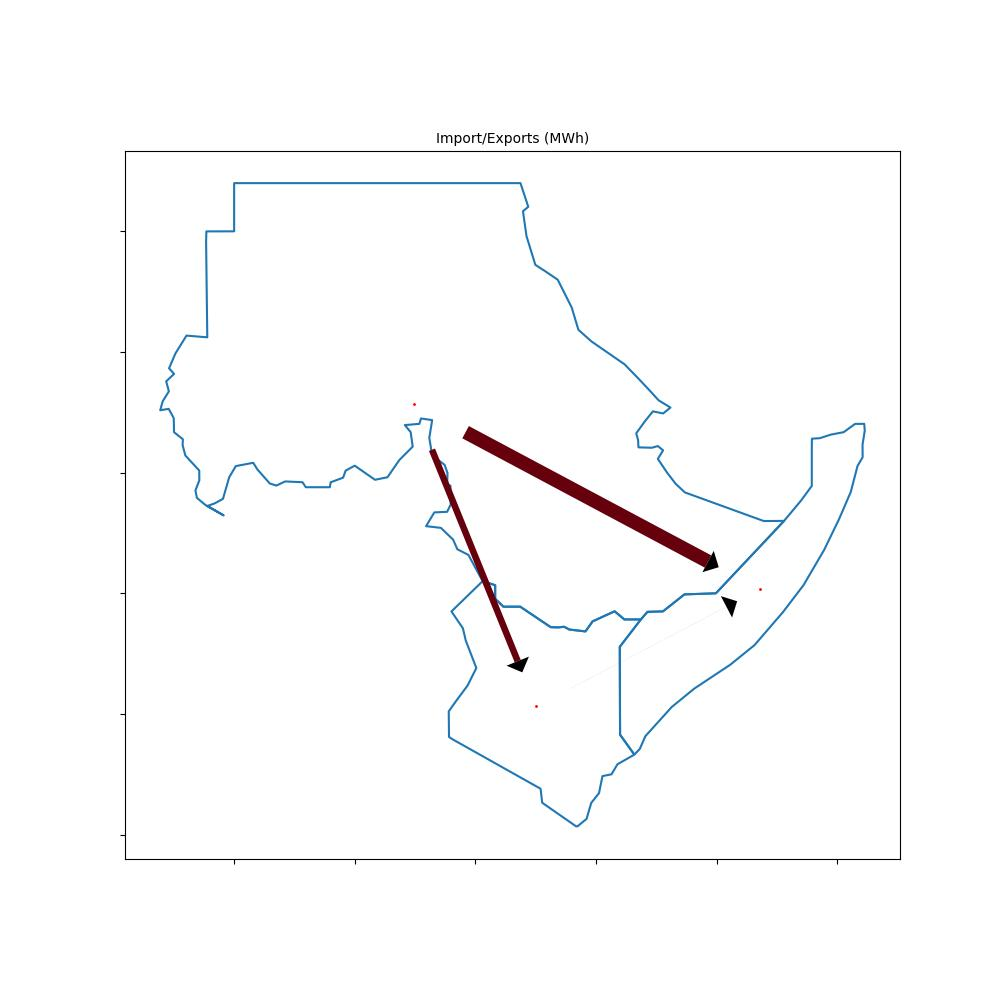
\includegraphics[width=\textwidth,keepaspectratio]{\home\Plan4Res\P4R3\p4r-env\bin\..\data\local\LoR_Madrid\results_simul\IMG\MeanFlows.jpeg}
\caption{Map of Mean Flows (MWh)}
\label{fig:MeanFlows.jpeg}
\end{figure}
\chapter{Detailed Results on Scenario 0}
\newpage\section{RoGonDor}
\subsection{Results on week 2031-01-12 to 2031-01-18}
\subsubsection{Electricity Generation}
\begin{figure}[H]
\centering
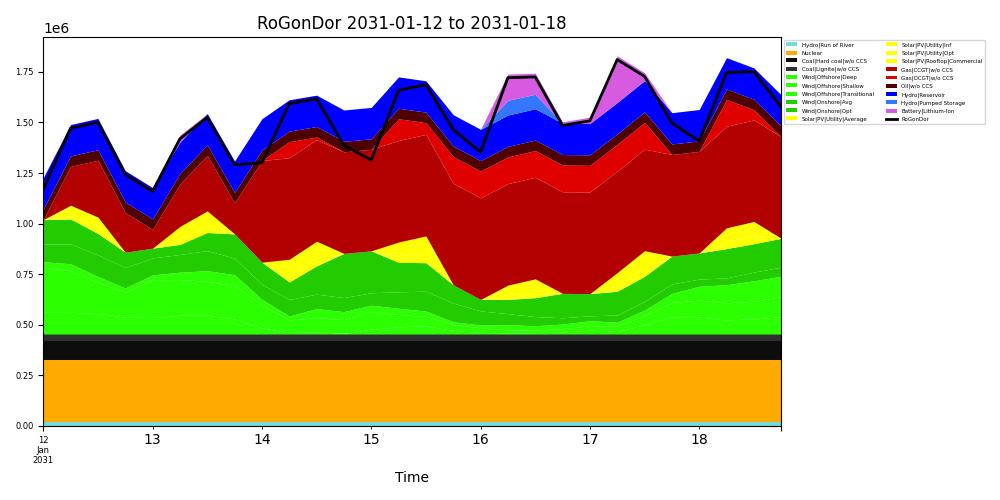
\includegraphics[width=\textwidth,keepaspectratio]{\home\Plan4Res\P4R3\p4r-env\bin\..\data\local\LoR_Madrid\results_simul\IMG\Scenario_0_StackedActivePower_RoGonDor2031-01-12.jpeg}
\caption{Electricity Generation in RoGonDor (MWh) from 2031-01-12 to 2031-01-18}
\label{fig:Scenario_0_StackedActivePower_RoGonDor2031-01-12.jpeg}
\end{figure}
\subsubsection{Marginal Cost}
\begin{figure}[H]
\centering
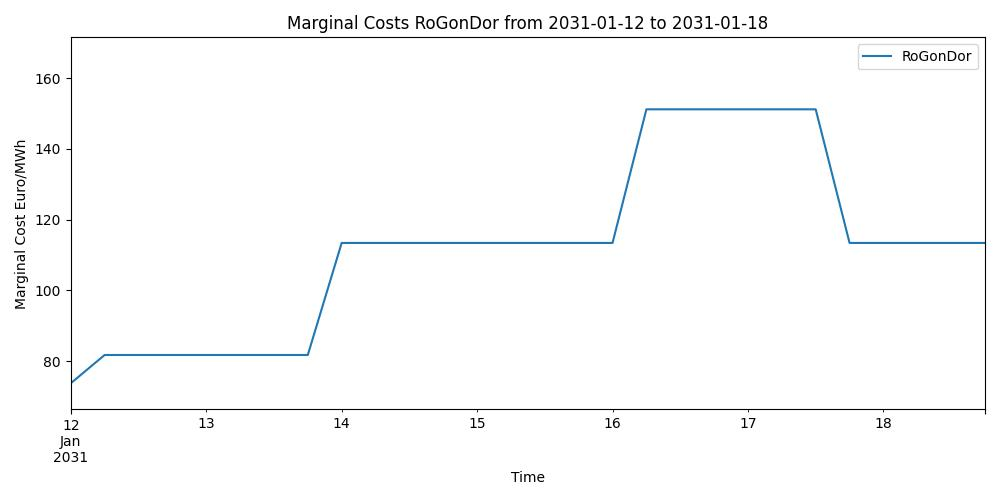
\includegraphics[width=\textwidth,keepaspectratio]{\home\Plan4Res\P4R3\p4r-env\bin\..\data\local\LoR_Madrid\results_simul\IMG\Scenario_0_CmarAPD_RoGonDor2031-01-12.jpeg}
\caption{Marginal Costs inRoGonDor (Euro/MWh) from 2031-01-12 to 2031-01-18}
\label{fig:Scenario_0_CmarAPD_RoGonDor2031-01-12.jpeg}
\end{figure}
\subsection{Global Results (from2030-07-02 to 2031-06-30)}
\subsubsection{Demand Marginal Cost}
\begin{figure}[H]
\centering
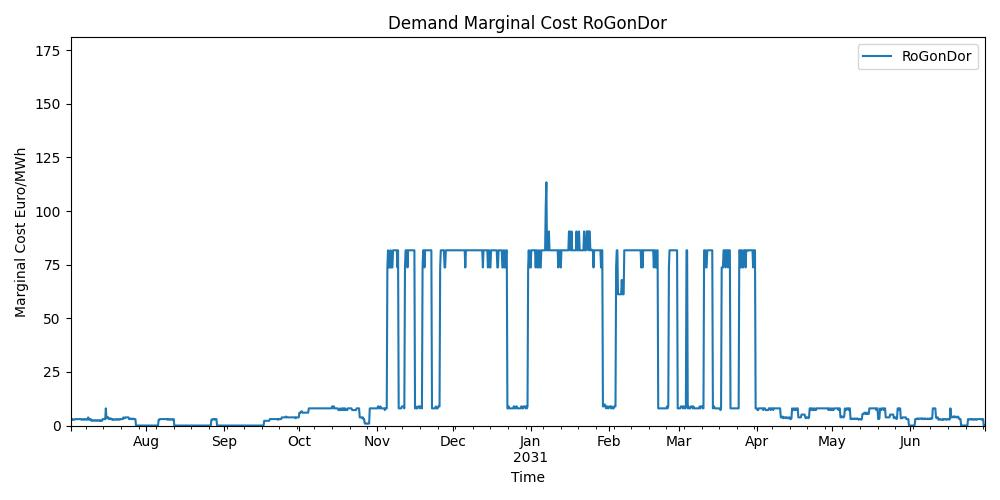
\includegraphics[width=\textwidth,keepaspectratio]{\home\Plan4Res\P4R3\p4r-env\bin\..\data\local\LoR_Madrid\results_simul\IMG\Scenario_0_MarginalCostDemand_RoGonDor2030-07-02.jpeg}
\caption{Marginal Cost Demand (Euro/MWh)}
\label{fig:Scenario_0_MarginalCostDemand_RoGonDor2030-07-02.jpeg}
\end{figure}
\subsubsection{Reservoir Storages}
\begin{figure}[H]
\centering
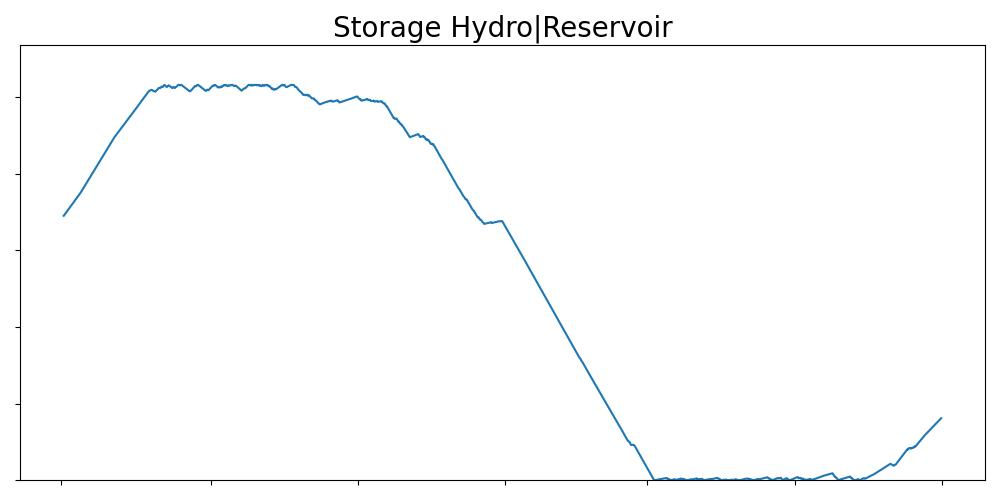
\includegraphics[width=\textwidth,keepaspectratio]{\home\Plan4Res\P4R3\p4r-env\bin\..\data\local\LoR_Madrid\results_simul\IMG\Scenario_0_Volume_Reservoir_RoGonDor2030-07-02.jpeg}
\caption{Reservoir storage level in RoGonDor (MWh)}
\label{fig:Scenario_0_Volume_Reservoir_RoGonDor2030-07-02.jpeg}
\end{figure}
\subsubsection{Pumped Storage Storages}
\begin{figure}[H]
\centering
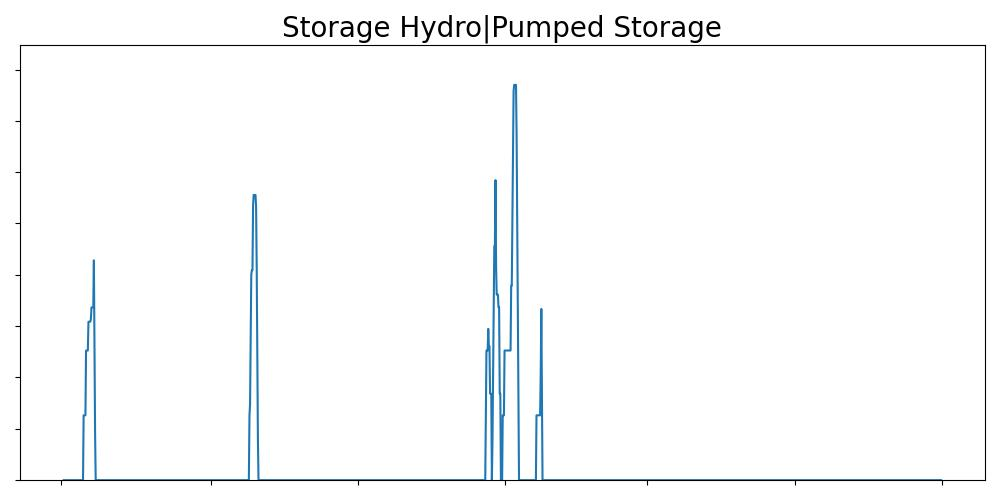
\includegraphics[width=\textwidth,keepaspectratio]{\home\Plan4Res\P4R3\p4r-env\bin\..\data\local\LoR_Madrid\results_simul\IMG\Scenario_0_Volume_PumpedStorage_RoGonDor2030-07-02.jpeg}
\caption{PumpedStorage storage level in RoGonDor (MWh)}
\label{fig:Scenario_0_Volume_PumpedStorage_RoGonDor2030-07-02.jpeg}
\end{figure}
\subsubsection{Batteries Storages}
\begin{figure}[H]
\centering
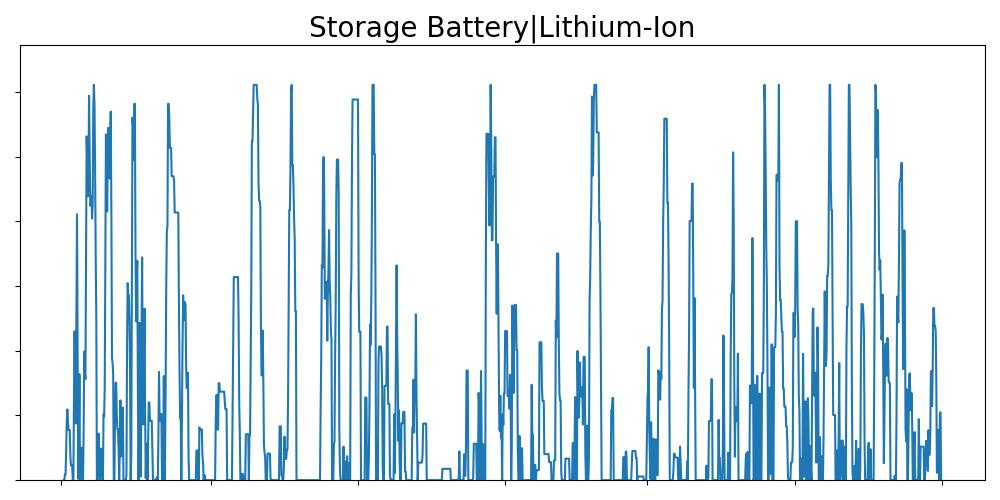
\includegraphics[width=\textwidth,keepaspectratio]{\home\Plan4Res\P4R3\p4r-env\bin\..\data\local\LoR_Madrid\results_simul\IMG\Scenario_0_Volume_Battery_RoGonDor2030-07-02.jpeg}
\caption{Battery storage level in RoGonDor (MWh)}
\label{fig:Scenario_0_Volume_Battery_RoGonDor2030-07-02.jpeg}
\end{figure}
\begin{figure}[H]
\centering
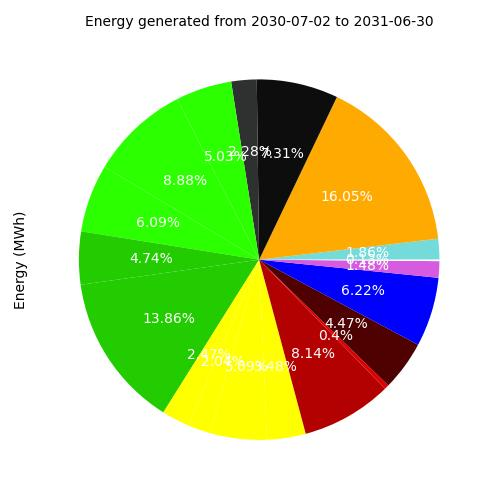
\includegraphics[width=\textwidth,keepaspectratio]{\home\Plan4Res\P4R3\p4r-env\bin\..\data\local\LoR_Madrid\results_simul\IMG\Scenario_0_Pie_RoGonDor2030-07-02.jpeg}
\caption{Energy Pie in RoGonDor}
\label{fig:Scenario_0_Pie_RoGonDor2030-07-02.jpeg}
\end{figure}
15 Hours with Loss of Load

\subsection{Costs}

Total Cost without Bellman Value=0.0
\newpage\section{DolAmroth}
\subsection{Results on week 2031-01-12 to 2031-01-18}
\subsubsection{Electricity Generation}
\begin{figure}[H]
\centering
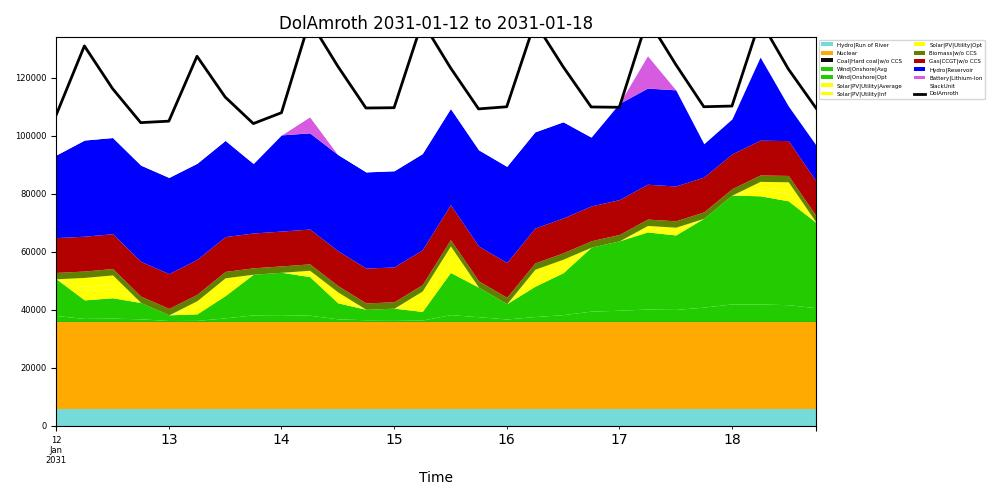
\includegraphics[width=\textwidth,keepaspectratio]{\home\Plan4Res\P4R3\p4r-env\bin\..\data\local\LoR_Madrid\results_simul\IMG\Scenario_0_StackedActivePower_DolAmroth2031-01-12.jpeg}
\caption{Electricity Generation in DolAmroth (MWh) from 2031-01-12 to 2031-01-18}
\label{fig:Scenario_0_StackedActivePower_DolAmroth2031-01-12.jpeg}
\end{figure}
\subsubsection{Marginal Cost}
\begin{figure}[H]
\centering
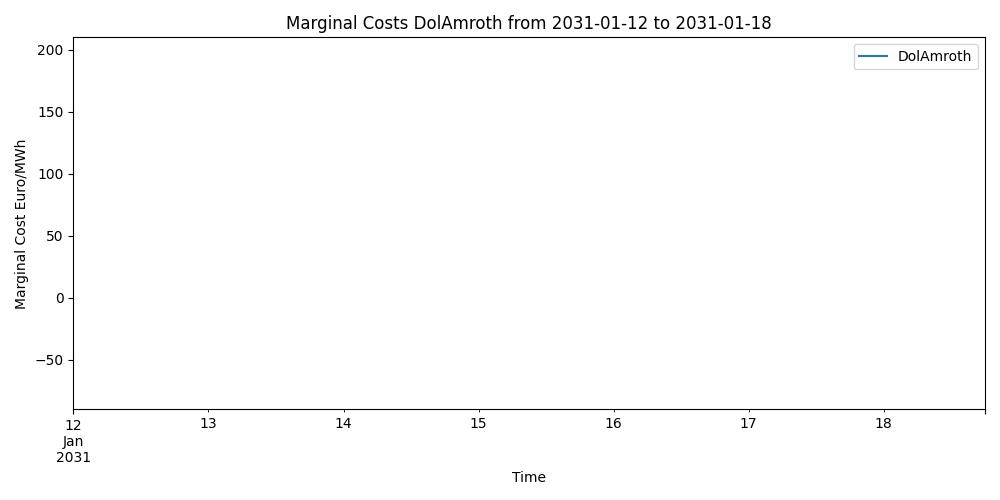
\includegraphics[width=\textwidth,keepaspectratio]{\home\Plan4Res\P4R3\p4r-env\bin\..\data\local\LoR_Madrid\results_simul\IMG\Scenario_0_CmarAPD_DolAmroth2031-01-12.jpeg}
\caption{Marginal Costs inDolAmroth (Euro/MWh) from 2031-01-12 to 2031-01-18}
\label{fig:Scenario_0_CmarAPD_DolAmroth2031-01-12.jpeg}
\end{figure}
\subsection{Global Results (from2030-07-02 to 2031-06-30)}
\subsubsection{Demand Marginal Cost}
\begin{figure}[H]
\centering
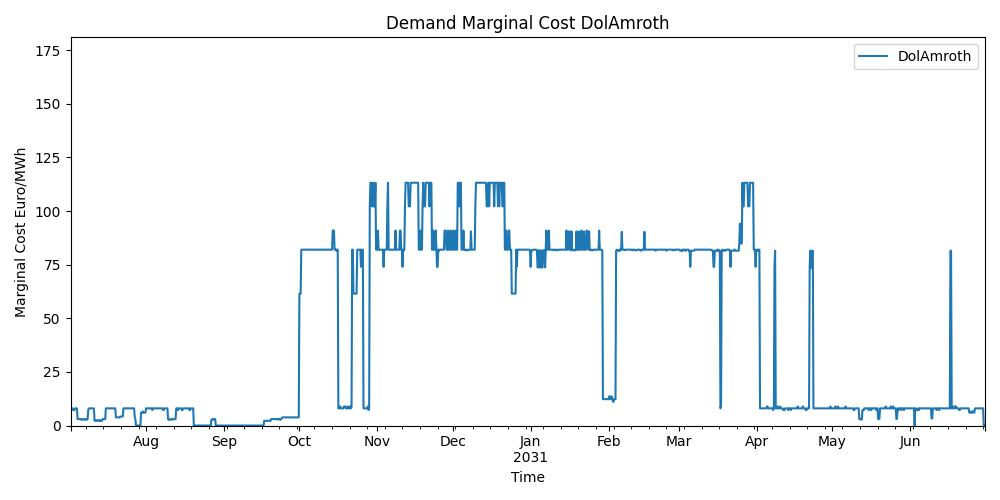
\includegraphics[width=\textwidth,keepaspectratio]{\home\Plan4Res\P4R3\p4r-env\bin\..\data\local\LoR_Madrid\results_simul\IMG\Scenario_0_MarginalCostDemand_DolAmroth2030-07-02.jpeg}
\caption{Marginal Cost Demand (Euro/MWh)}
\label{fig:Scenario_0_MarginalCostDemand_DolAmroth2030-07-02.jpeg}
\end{figure}
\subsubsection{Reservoir Storages}
\begin{figure}[H]
\centering
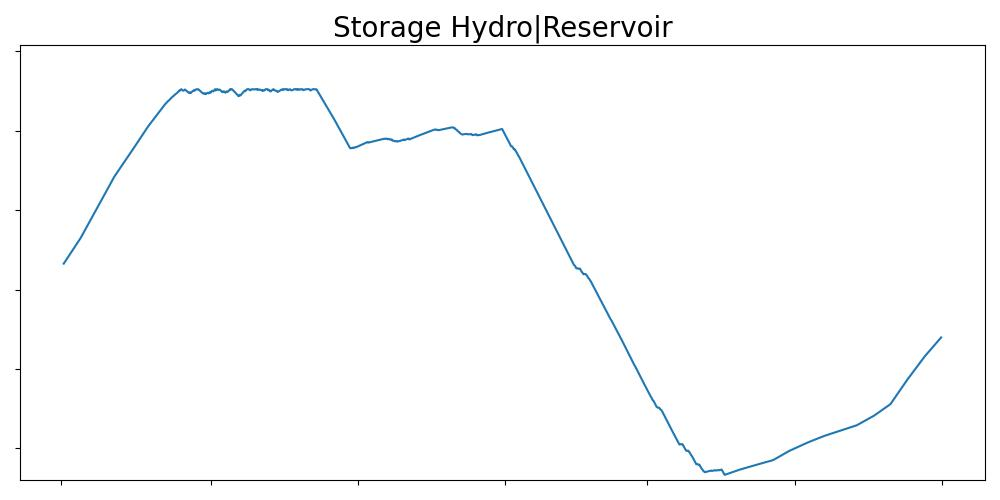
\includegraphics[width=\textwidth,keepaspectratio]{\home\Plan4Res\P4R3\p4r-env\bin\..\data\local\LoR_Madrid\results_simul\IMG\Scenario_0_Volume_Reservoir_DolAmroth2030-07-02.jpeg}
\caption{Reservoir storage level in DolAmroth (MWh)}
\label{fig:Scenario_0_Volume_Reservoir_DolAmroth2030-07-02.jpeg}
\end{figure}
\subsubsection{Pumped Storage Storages}
\begin{figure}[H]
\centering
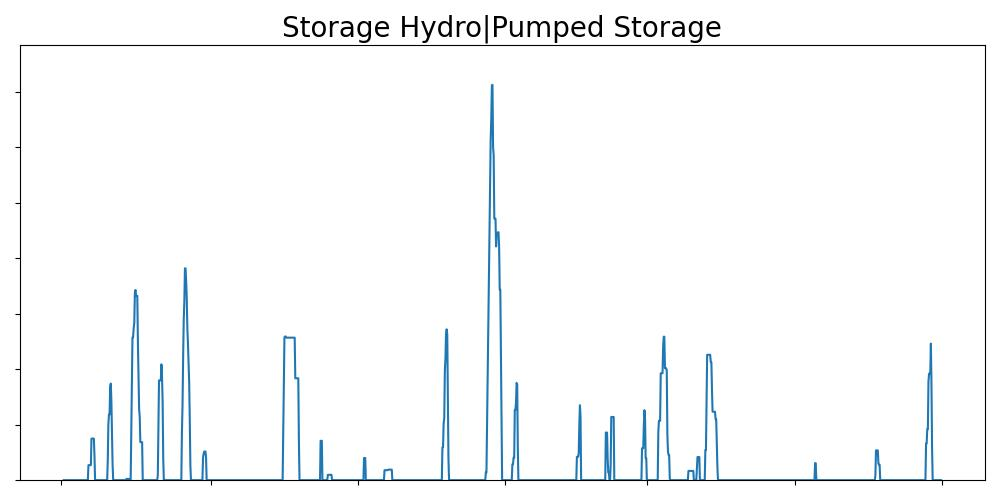
\includegraphics[width=\textwidth,keepaspectratio]{\home\Plan4Res\P4R3\p4r-env\bin\..\data\local\LoR_Madrid\results_simul\IMG\Scenario_0_Volume_PumpedStorage_DolAmroth2030-07-02.jpeg}
\caption{PumpedStorage storage level in DolAmroth (MWh)}
\label{fig:Scenario_0_Volume_PumpedStorage_DolAmroth2030-07-02.jpeg}
\end{figure}
\subsubsection{Batteries Storages}
\begin{figure}[H]
\centering
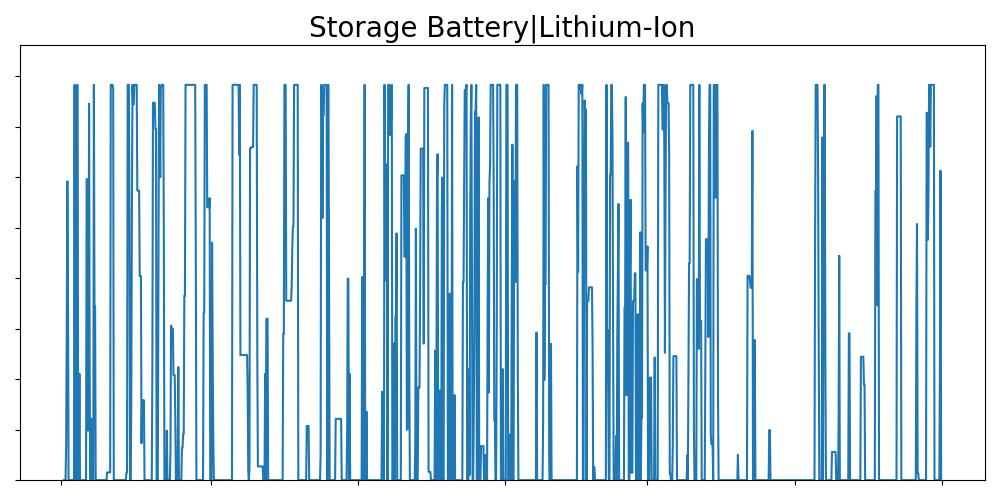
\includegraphics[width=\textwidth,keepaspectratio]{\home\Plan4Res\P4R3\p4r-env\bin\..\data\local\LoR_Madrid\results_simul\IMG\Scenario_0_Volume_Battery_DolAmroth2030-07-02.jpeg}
\caption{Battery storage level in DolAmroth (MWh)}
\label{fig:Scenario_0_Volume_Battery_DolAmroth2030-07-02.jpeg}
\end{figure}
\begin{figure}[H]
\centering
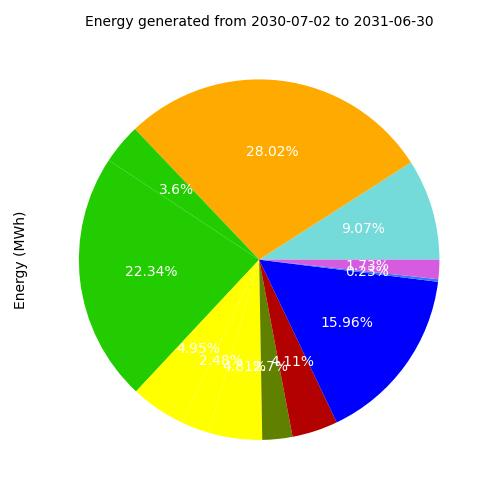
\includegraphics[width=\textwidth,keepaspectratio]{\home\Plan4Res\P4R3\p4r-env\bin\..\data\local\LoR_Madrid\results_simul\IMG\Scenario_0_Pie_DolAmroth2030-07-02.jpeg}
\caption{Energy Pie in DolAmroth}
\label{fig:Scenario_0_Pie_DolAmroth2030-07-02.jpeg}
\end{figure}
204 Hours with Loss of Load

\subsection{Costs}

Total Cost without Bellman Value=0.0
\newpage\section{Harad}
\subsection{Results on week 2031-01-12 to 2031-01-18}
\subsubsection{Electricity Generation}
\begin{figure}[H]
\centering
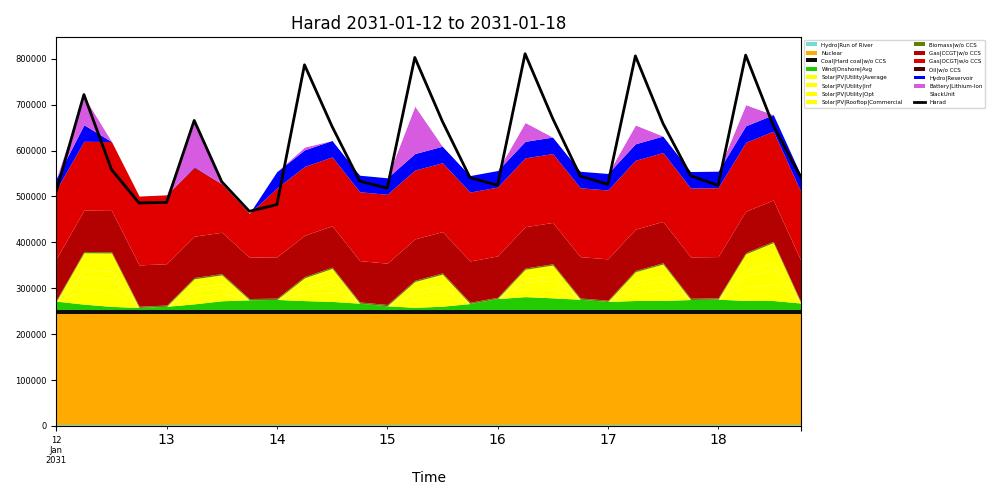
\includegraphics[width=\textwidth,keepaspectratio]{\home\Plan4Res\P4R3\p4r-env\bin\..\data\local\LoR_Madrid\results_simul\IMG\Scenario_0_StackedActivePower_Harad2031-01-12.jpeg}
\caption{Electricity Generation in Harad (MWh) from 2031-01-12 to 2031-01-18}
\label{fig:Scenario_0_StackedActivePower_Harad2031-01-12.jpeg}
\end{figure}
\subsubsection{Marginal Cost}
\begin{figure}[H]
\centering
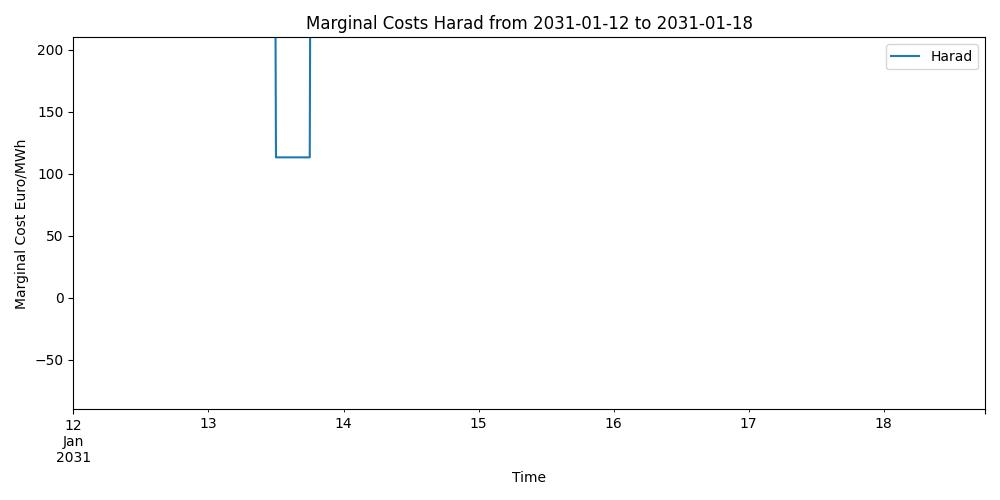
\includegraphics[width=\textwidth,keepaspectratio]{\home\Plan4Res\P4R3\p4r-env\bin\..\data\local\LoR_Madrid\results_simul\IMG\Scenario_0_CmarAPD_Harad2031-01-12.jpeg}
\caption{Marginal Costs inHarad (Euro/MWh) from 2031-01-12 to 2031-01-18}
\label{fig:Scenario_0_CmarAPD_Harad2031-01-12.jpeg}
\end{figure}
\subsection{Global Results (from2030-07-02 to 2031-06-30)}
\subsubsection{Demand Marginal Cost}
\begin{figure}[H]
\centering
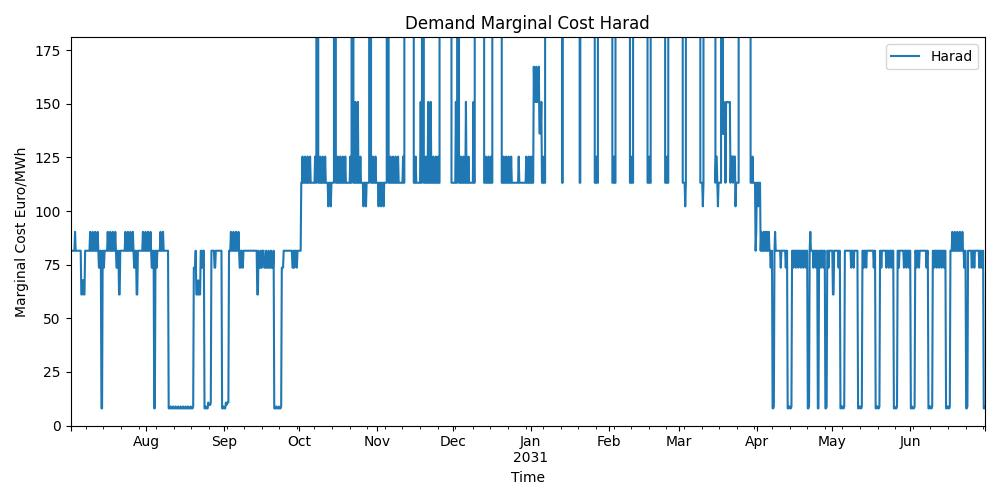
\includegraphics[width=\textwidth,keepaspectratio]{\home\Plan4Res\P4R3\p4r-env\bin\..\data\local\LoR_Madrid\results_simul\IMG\Scenario_0_MarginalCostDemand_Harad2030-07-02.jpeg}
\caption{Marginal Cost Demand (Euro/MWh)}
\label{fig:Scenario_0_MarginalCostDemand_Harad2030-07-02.jpeg}
\end{figure}
\subsubsection{Reservoir Storages}
\begin{figure}[H]
\centering
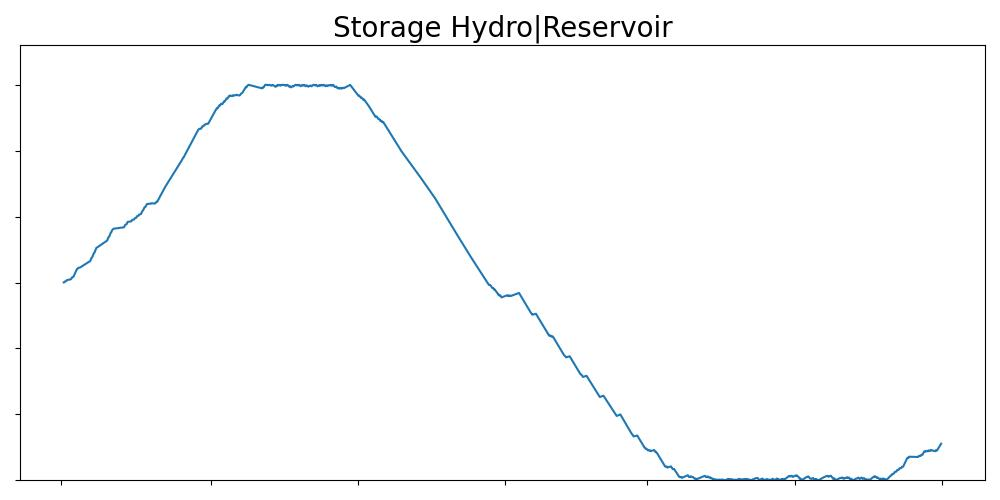
\includegraphics[width=\textwidth,keepaspectratio]{\home\Plan4Res\P4R3\p4r-env\bin\..\data\local\LoR_Madrid\results_simul\IMG\Scenario_0_Volume_Reservoir_Harad2030-07-02.jpeg}
\caption{Reservoir storage level in Harad (MWh)}
\label{fig:Scenario_0_Volume_Reservoir_Harad2030-07-02.jpeg}
\end{figure}
\subsubsection{Pumped Storage Storages}
\begin{figure}[H]
\centering
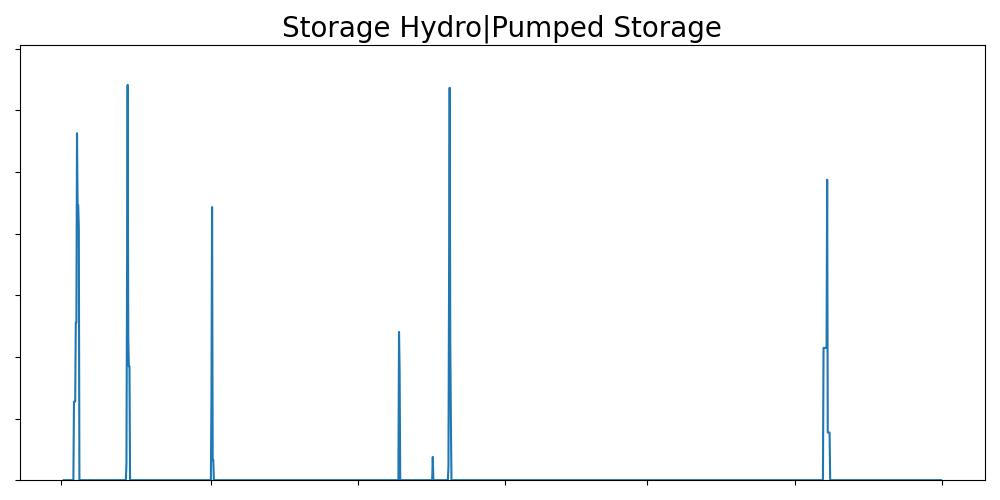
\includegraphics[width=\textwidth,keepaspectratio]{\home\Plan4Res\P4R3\p4r-env\bin\..\data\local\LoR_Madrid\results_simul\IMG\Scenario_0_Volume_PumpedStorage_Harad2030-07-02.jpeg}
\caption{PumpedStorage storage level in Harad (MWh)}
\label{fig:Scenario_0_Volume_PumpedStorage_Harad2030-07-02.jpeg}
\end{figure}
\subsubsection{Batteries Storages}
\begin{figure}[H]
\centering
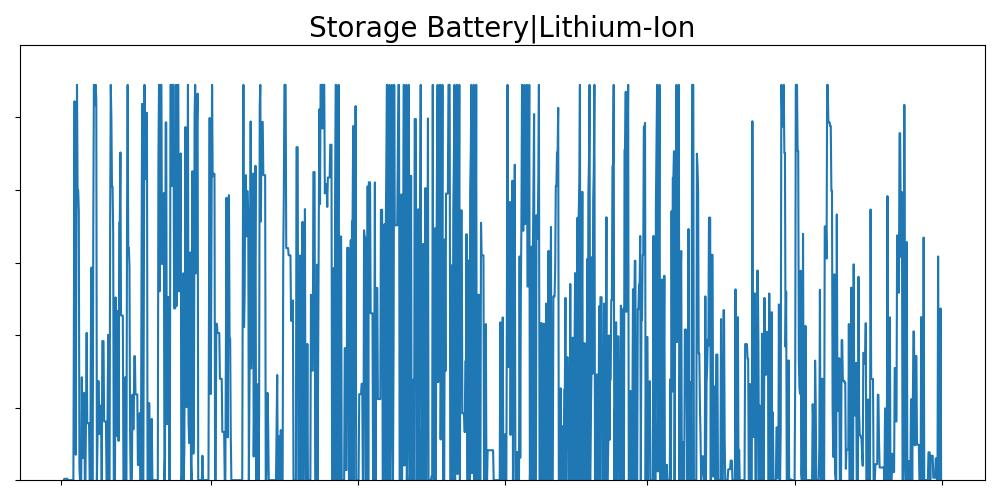
\includegraphics[width=\textwidth,keepaspectratio]{\home\Plan4Res\P4R3\p4r-env\bin\..\data\local\LoR_Madrid\results_simul\IMG\Scenario_0_Volume_Battery_Harad2030-07-02.jpeg}
\caption{Battery storage level in Harad (MWh)}
\label{fig:Scenario_0_Volume_Battery_Harad2030-07-02.jpeg}
\end{figure}
\begin{figure}[H]
\centering
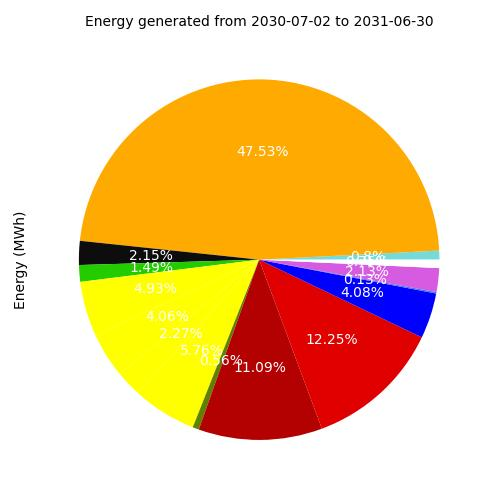
\includegraphics[width=\textwidth,keepaspectratio]{\home\Plan4Res\P4R3\p4r-env\bin\..\data\local\LoR_Madrid\results_simul\IMG\Scenario_0_Pie_Harad2030-07-02.jpeg}
\caption{Energy Pie in Harad}
\label{fig:Scenario_0_Pie_Harad2030-07-02.jpeg}
\end{figure}
92 Hours with Loss of Load

\subsection{Costs}

Total Cost without Bellman Value=0.0
\newpage\section{Synthesis All Countries}
\subsection{Costs}
Total Cost for all countries, without Bellman Values=0.0 Euros

Total Cost for all countries, with Bellman Values=0.0 Euros

\begin{figure}[H]
\centering
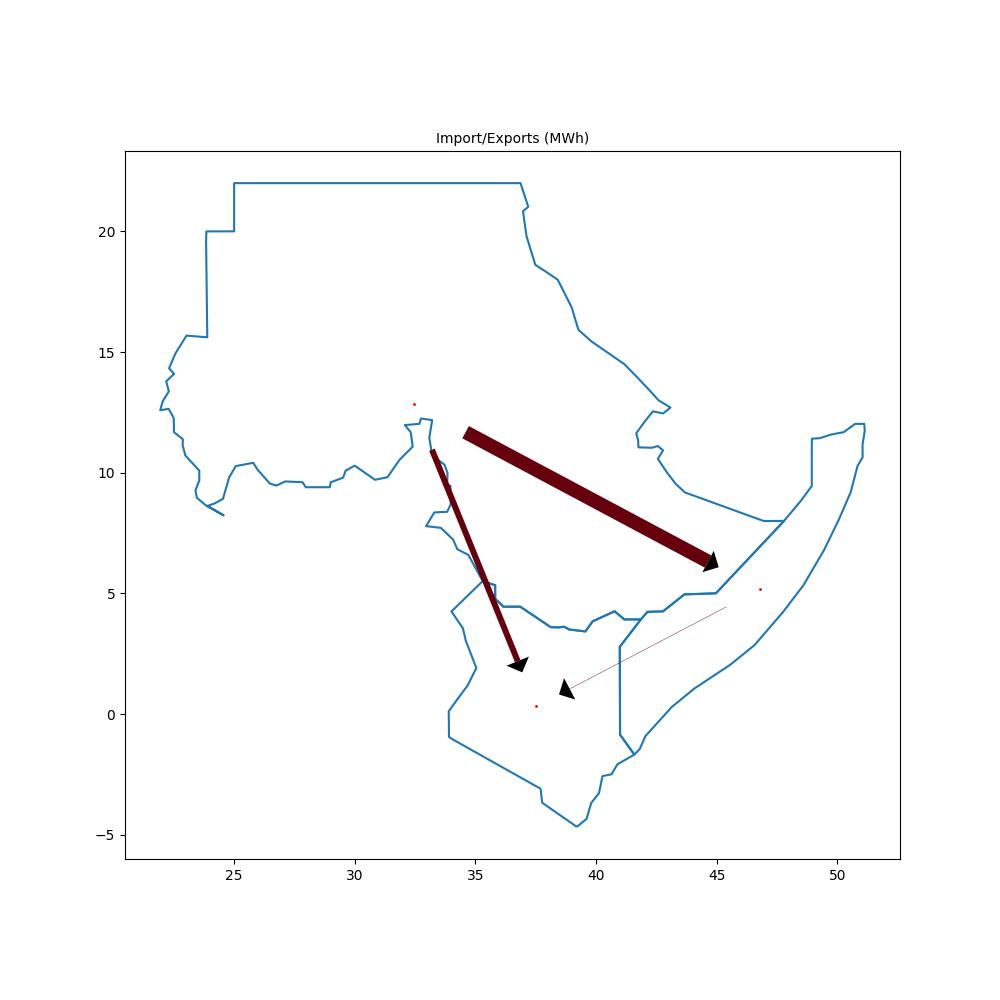
\includegraphics[width=\textwidth,keepaspectratio]{\home\Plan4Res\P4R3\p4r-env\bin\..\data\local\LoR_Madrid\results_simul\IMG\Scenario_0_ArrowImpExp.jpeg}
\caption{Map of Interconnection uses over the whole period (MWh)}
\label{fig:Scenario_0_ArrowImpExp.jpeg}
\end{figure}
\subsection{Energy generation}
\begin{figure}[H]
\centering
\includegraphics[width=\textwidth,keepaspectratio]{\home\Plan4Res\P4R3\p4r-env\bin\..\data\local\LoR_Madrid\results_simul\IMG\Scenario_ChloroMap-MeanEnergy.jpeg}
\caption{Map of energy generated for Scenario 0 (MWh)}
\label{fig:Scenario_ChloroMap-MeanEnergy.jpeg}
\end{figure}
\begin{figure}[H]
\centering
\includegraphics[width=\textwidth,keepaspectratio]{\home\Plan4Res\P4R3\p4r-env\bin\..\data\local\LoR_Madrid\results_simul\IMG\Scenario_EnergyPieEurope.jpeg}
\caption{Map of countries Energy Generated}
\label{fig:Scenario_EnergyPieEurope.jpeg}
\end{figure}
\subsection{CO2 Emissions}
\begin{figure}[H]
\centering
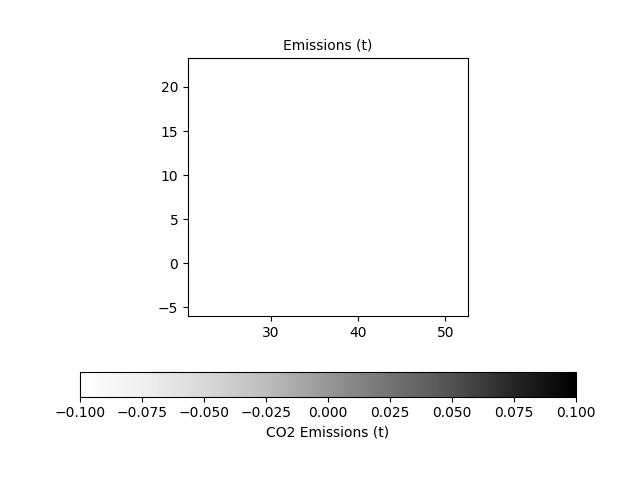
\includegraphics[width=\textwidth,keepaspectratio]{\home\Plan4Res\P4R3\p4r-env\bin\..\data\local\LoR_Madrid\results_simul\IMG\Scenario_ChloroMap-CO2.jpeg}
\caption{Map of Carbon Emissions (tons)}
\label{fig:Scenario_ChloroMap-CO2.jpeg}
\end{figure}
\end{document}